%!TEX root = Humanoids2013.tex
\section{Model--Free Application}

In this section we present an experimental application on a prototype of the hopping robot represented in Fig.~\ref{fig:Prototype}. The objective is to show that, even though the proposed method is analytical, it is directly applicable to existing systems whose model is not accurate or not available at all. Indeed, the optimization of the actuation parameters need to evaluate the function $f_a(\ddot x, \dot x, x, \ddot{q}, \dot{q}, q, t)$ and in~\eqref{eq:underact1_SEAplus} in case of SEA, or in \eqref{eq:underact_PEAplus} in case of PEA, in terms of the desired joint trajectories. However, in an experimental setup, as $f_a(\cdot)$ can also be directly measured from the real system by means of suitable sensors.  
To correctly the optimization procedure, it is sufficient to obtain the derivatives of the measured signal $f_a(t)$, which can be obtained by applying techniques such as e.g.~in~\cite{Fliess2003}.
Through the following experiment we are hence able to show that our method can be applied to systems whose model is unknown, i.e.~in a model--free fashion. 

% The procedure proposed in this paper is applied to the prototype of the hopping robot represented in Fig.~\ref{fig:Prototype} mainly to show that, nonetheless the method is based on the knowledge of the model of the mechanical system, it works well also using experimental data acquired directly from sensors suitable placed on the real system, i.e.~in a model--free fashion. 

The prototype of the planar elastic hopping robot represented in Fig.~\ref{fig:Prototype}. Referring to Fig.~\ref{fig:SaltarelloEsploso}, it has one leg which is composed of two links (1 and 2), three DoFs and it is linked to the frame through two non actuated DoFs  (3 and 4). All joints are provided with a contactless magnetic rotary position sensor (AS5045\footnote{\url{http://www.ams.com}}, colored in red). The two joints of the leg are actuated by DC geared motors (maxon DCX 22S\footnote{\url{http://dcx.maxonmotor.com}} with graphite brushes $24$ V, and planetary gearhead GPX22 with reduction ratio $83:1$, 5 and 6). The hopper is actuated by a SEA in the knee, while the other joint is stiff (see Fig.~\ref{fig:SaltarelloEsploso}).
The series elastic transmission 10 between the actuator 11 and the knee joint is composed of two rubber bands. 

Wheel 7 is placed at the extremity of the leg in order to reduce the effect of the friction component perpendicular to the direction of motion. To guarantee a vertical hopping, the leg has been constrained through a vertical linear guide 8. An electronic board\footnote{\url{http://www.naturalmotioninitiative.com/}} 9 has been used to acquire the measurements from the encoders and to implement a closed loop position control scheme tracking the desired trajectories (the controller furnishes input values at a frequency of $1$ kHz).
\begin{figure*}[!t]
\centering
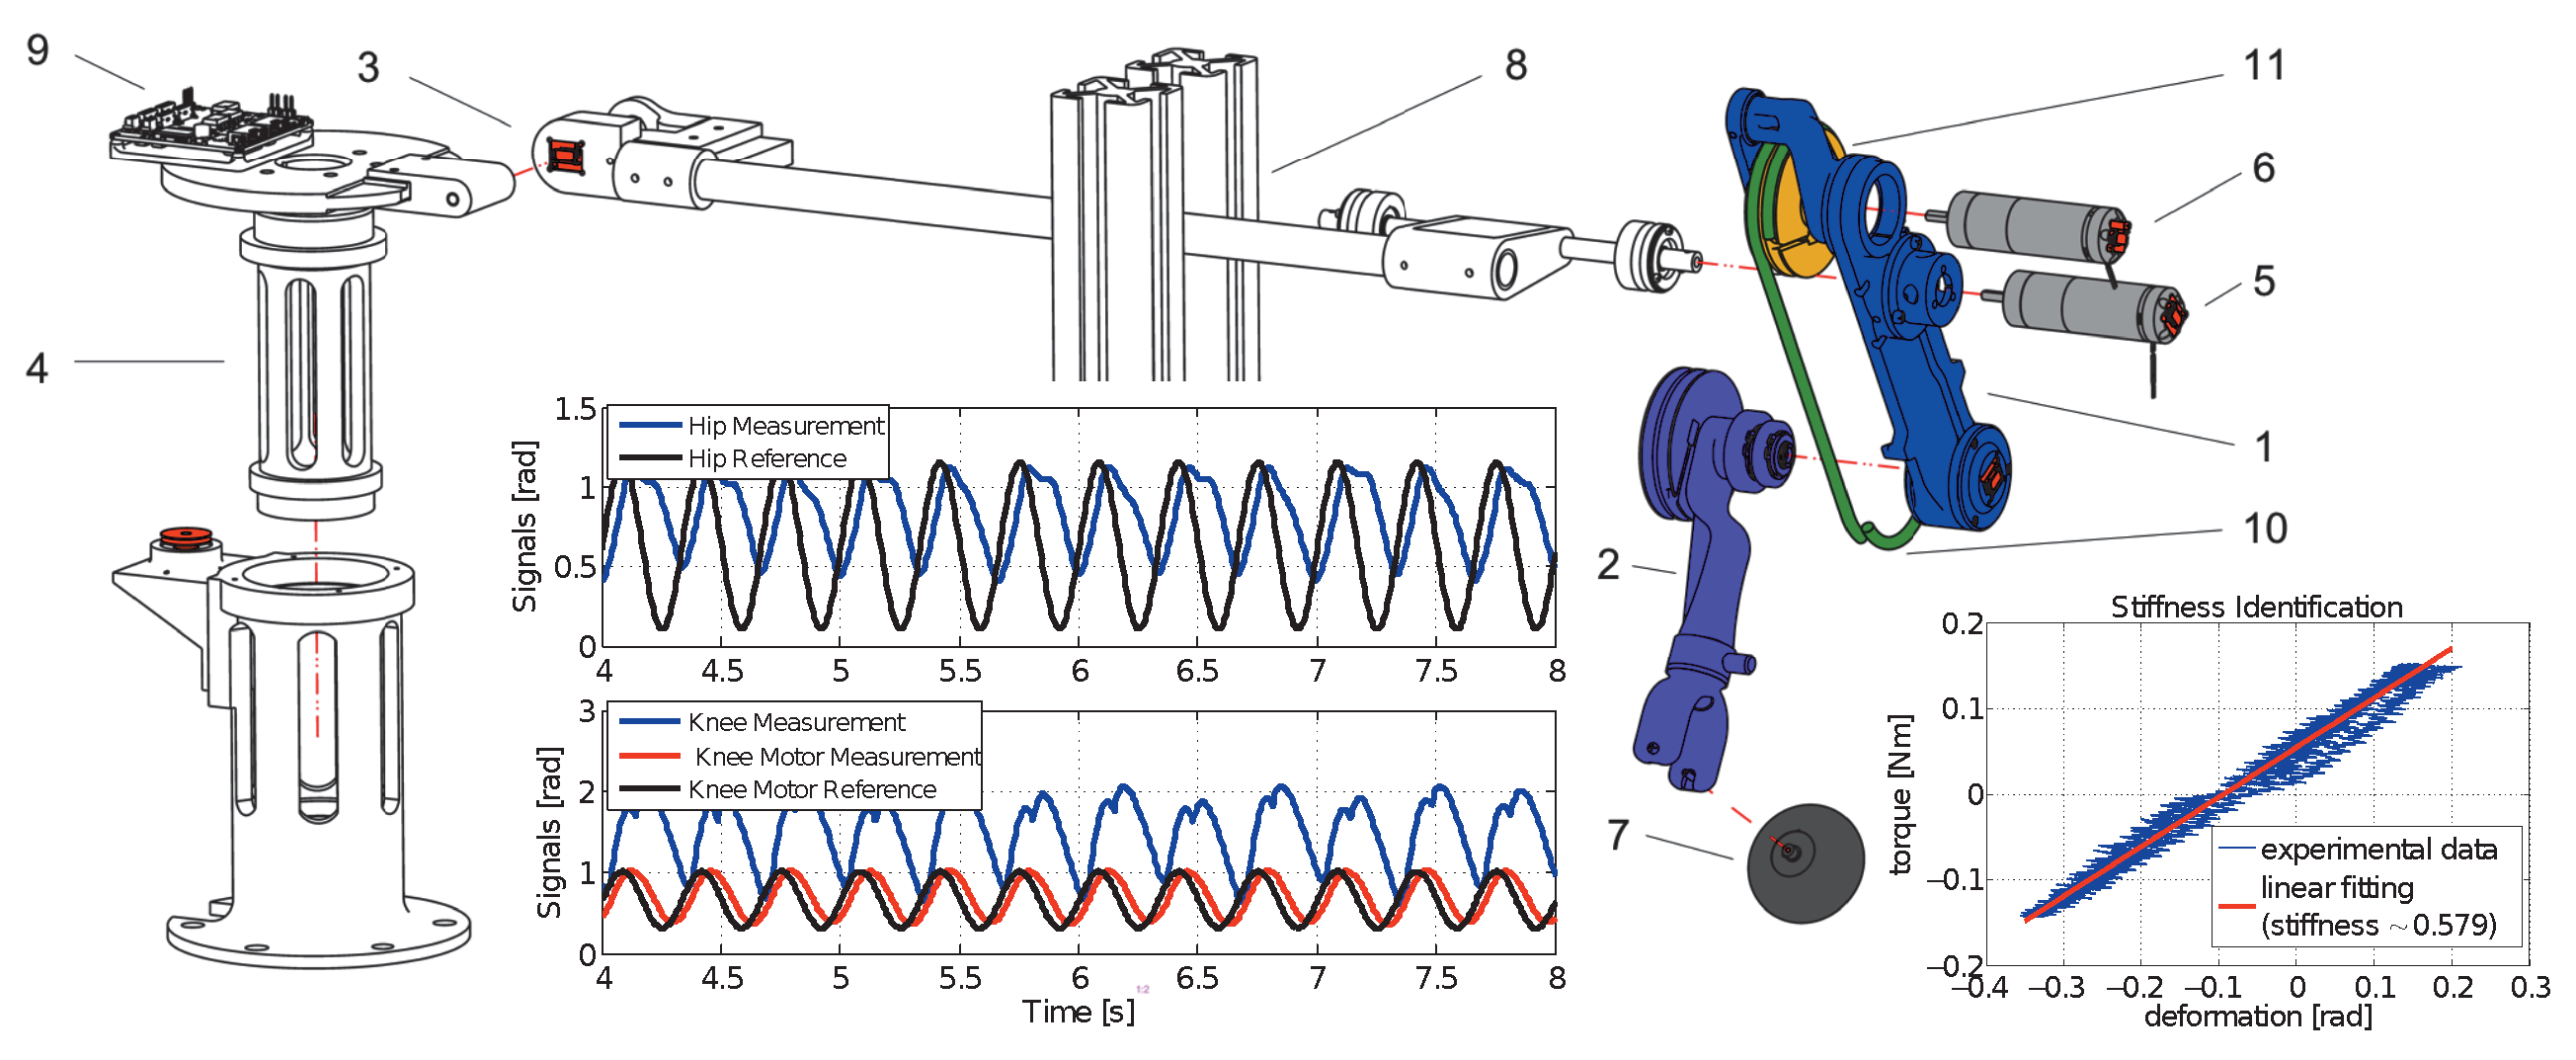
\includegraphics[width=0.89\textwidth]{dwg/SaltarelloEsploso}
\caption{Exploded 3D view of the hopping robot. The figure also shows the graphical values of torque and corresponding deformation used for stiffness identification. Moreover, in the center of the picture are reported reference signals and measured link trajectories.}
\label{fig:SaltarelloEsploso}
\end{figure*}

% \begin{figure}[!t]
% \centering
% 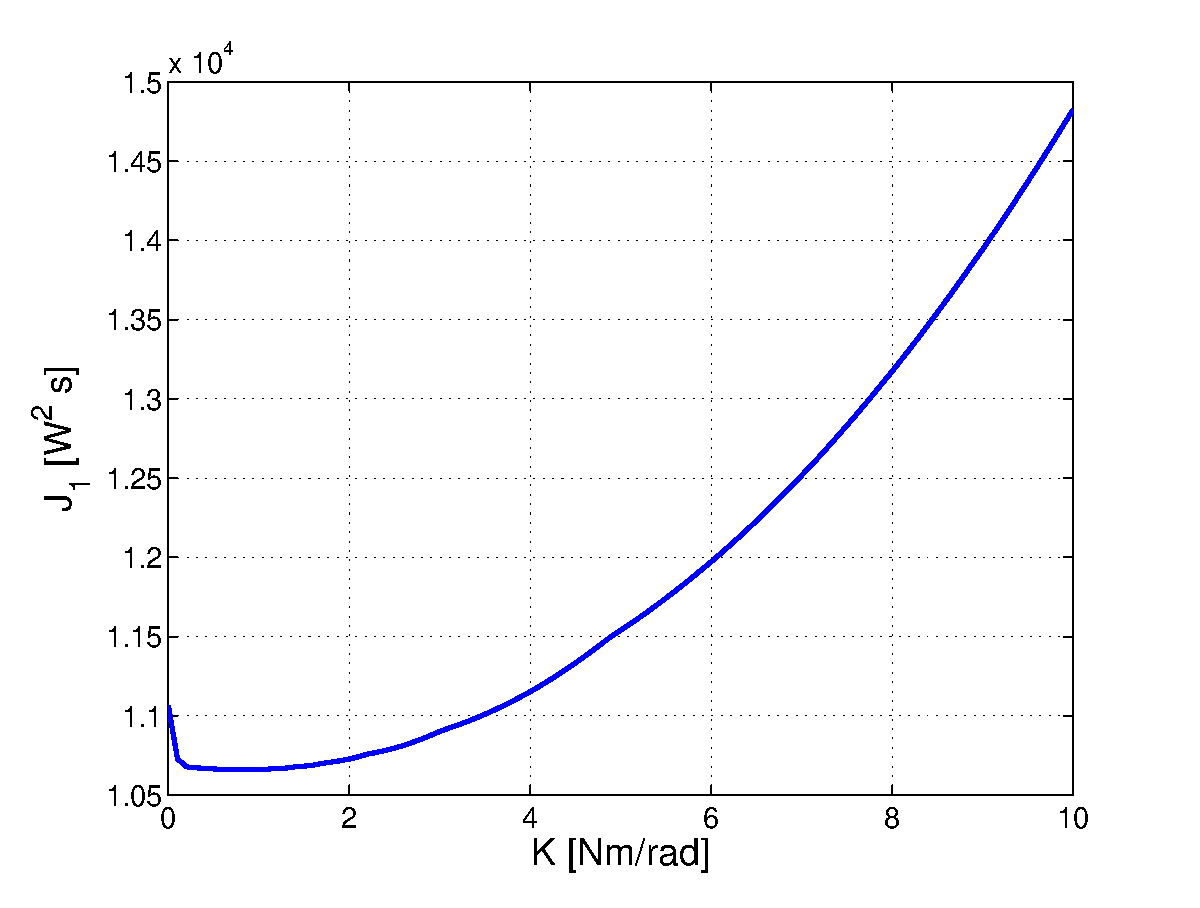
\includegraphics[width=0.9\columnwidth]{dwg/curveJ1pea}
% \caption{.}
% \label{fig:SaltarelloEsploso}
% \end{figure}
% 
% \begin{figure}[!t]
% \centering
% 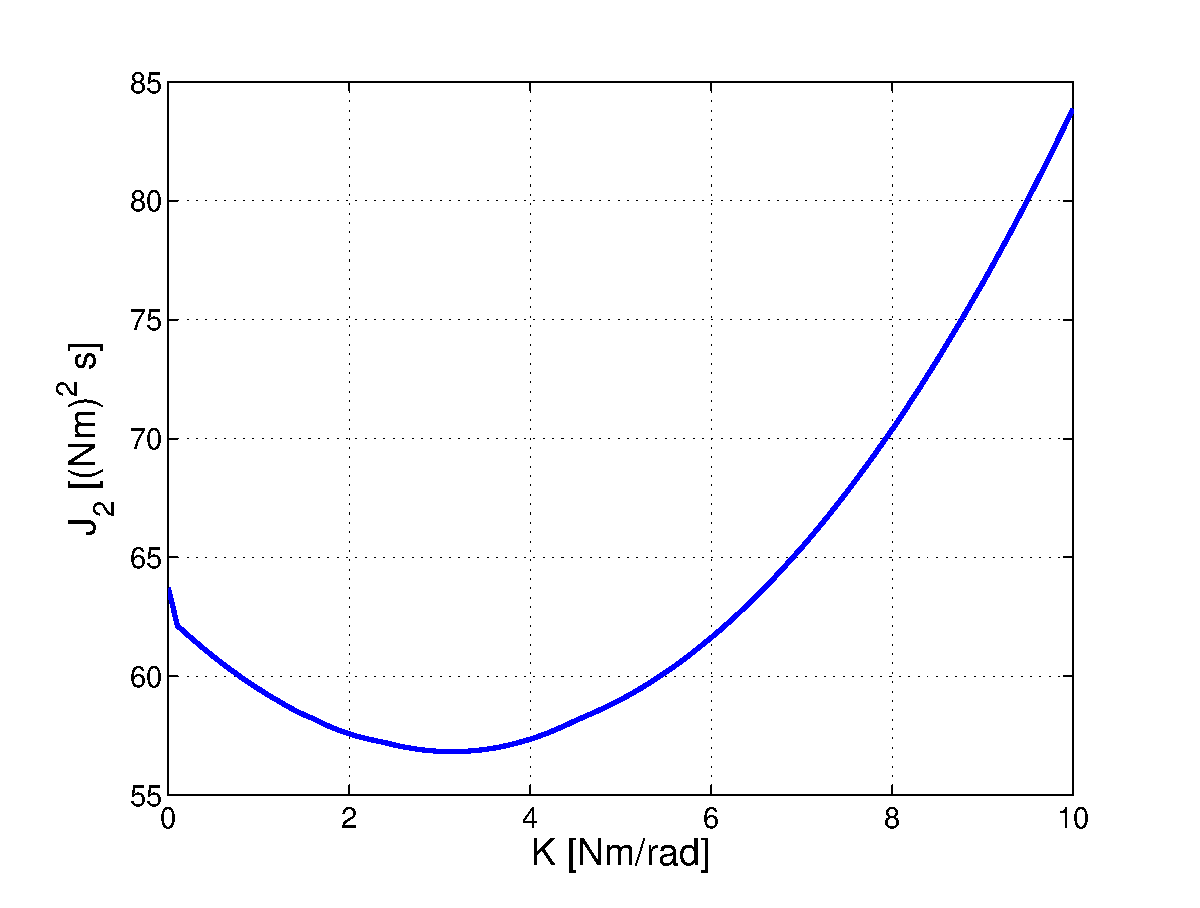
\includegraphics[width=1\columnwidth]{dwg/curveJ2pea}
% \caption{.}
% \label{fig:SaltarelloEsploso}
% \end{figure}

%%-%
\begin{figure*}[t]
\centering
\subfigure[Cost index $J_2$ for different values stiffness in case of SEAs.]{\label{fig:J2_SEA}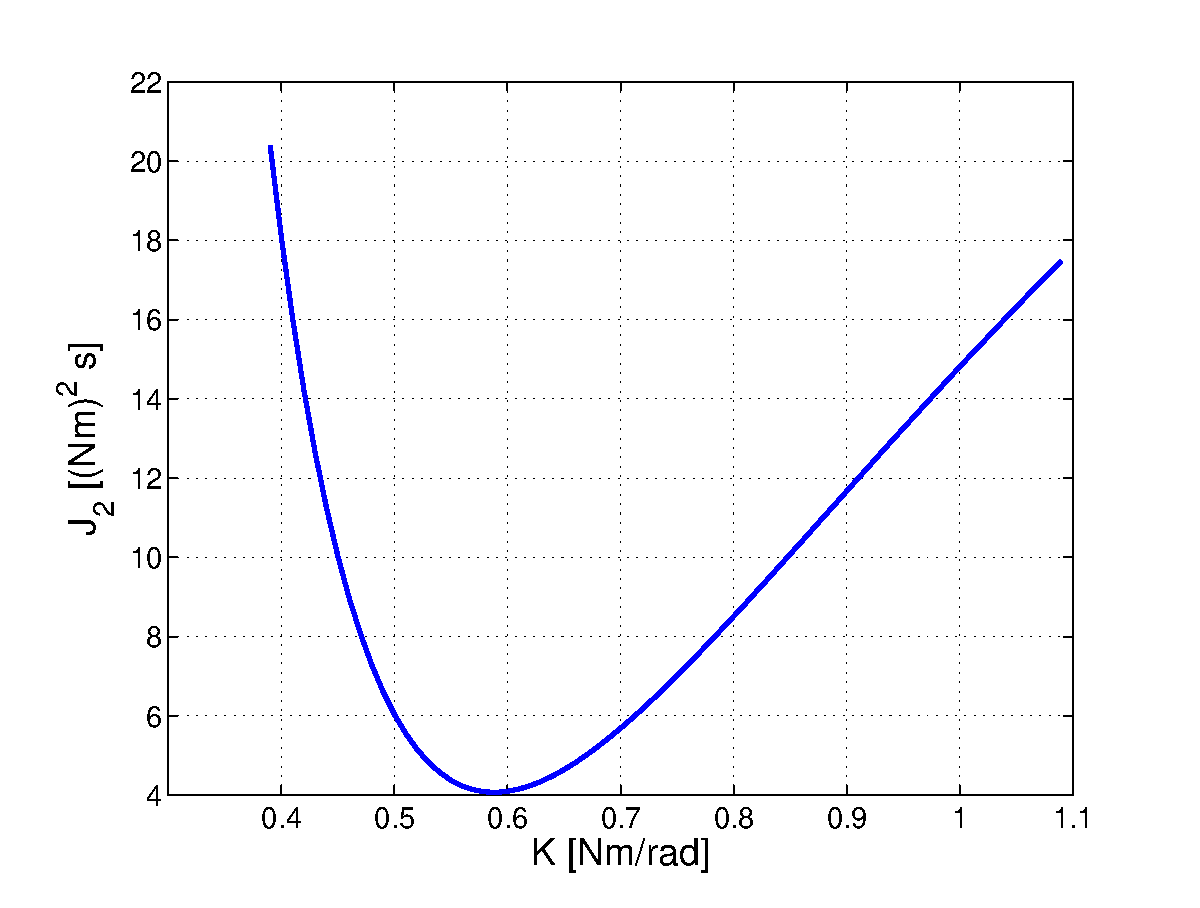
\includegraphics[width=0.5\columnwidth]{dwg/curveJ2sea}}
\subfigure[Cost index $J_2$ for different values stiffness in case of PEAs.]{\label{fig:J1_PEA}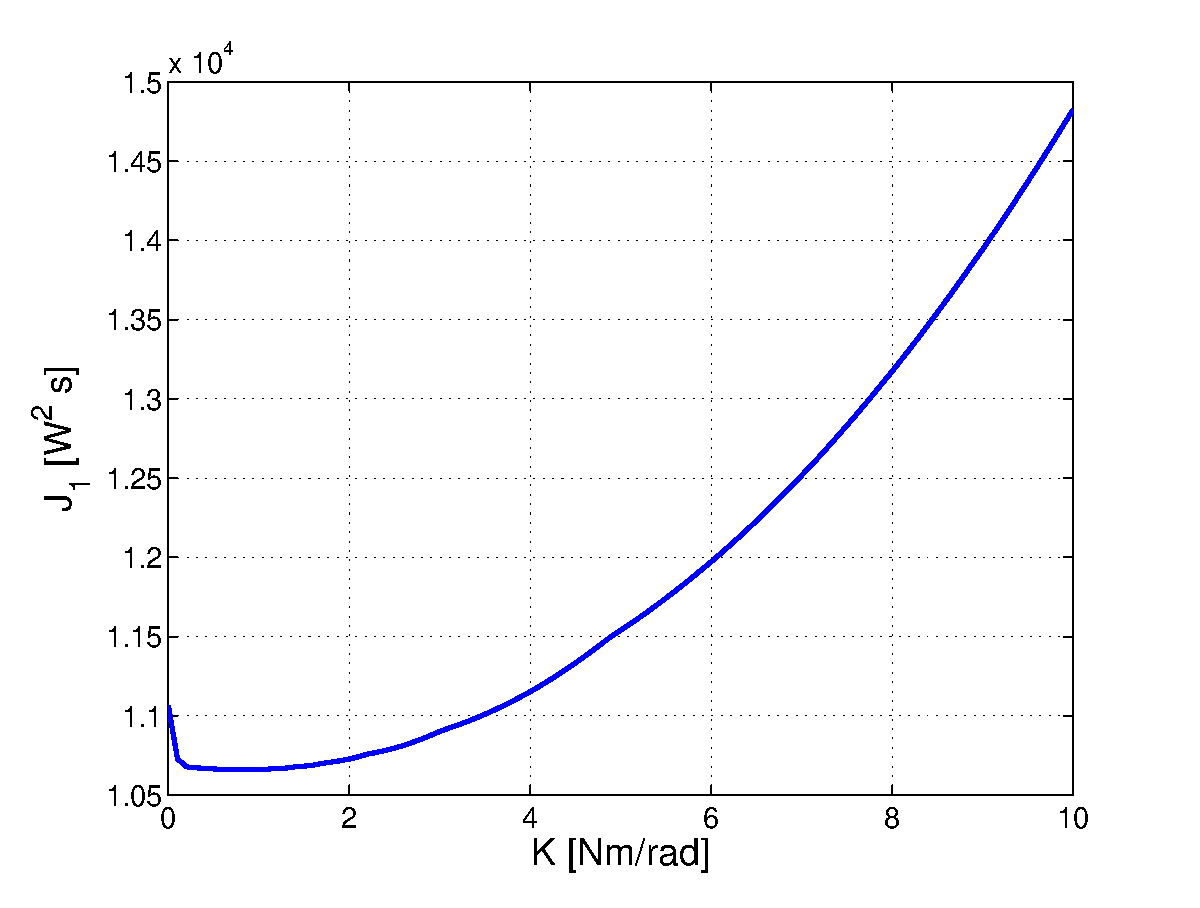
\includegraphics[width=0.5\columnwidth]{dwg/curveJ1pea}}
\subfigure[Cost index $J_1$ for different values stiffness in case of SEAs.]{\label{fig:J1_SEA}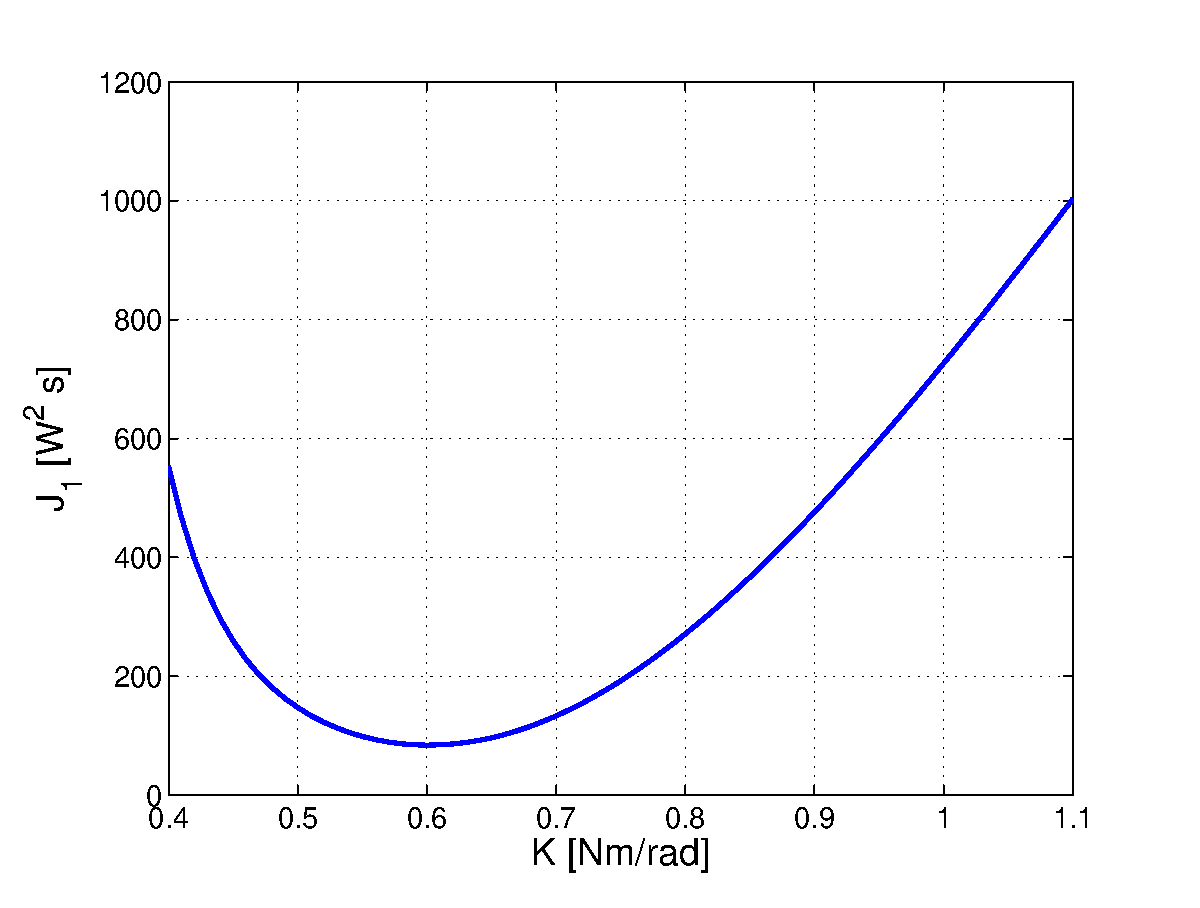
\includegraphics[width=0.5\columnwidth]{dwg/curveJ1sea}}
\subfigure[Cost index $J_1$ for different values stiffness in case of PEAs.]{\label{fig:J2_PEA}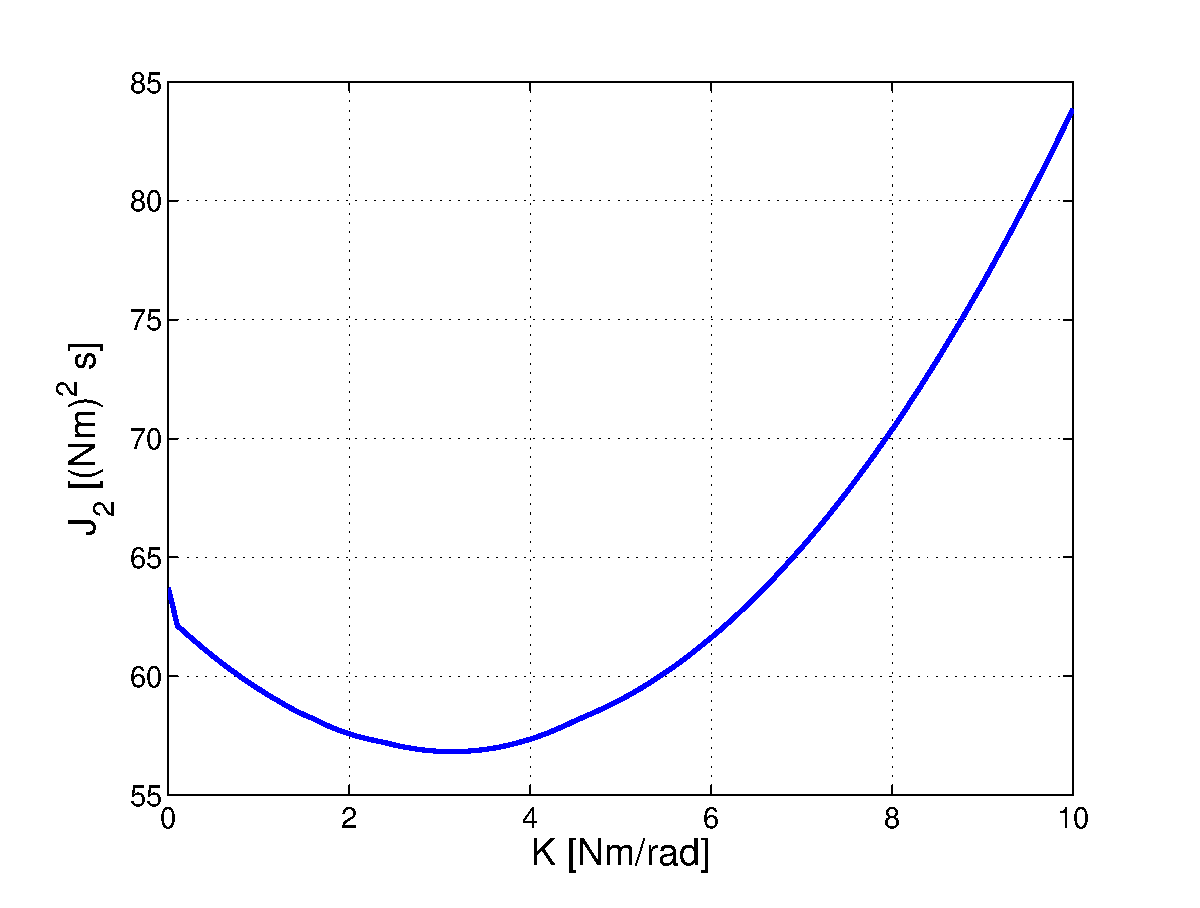
\includegraphics[width=0.5\columnwidth]{dwg/curveJ2pea}}
\caption{Cost indices $J_1$ and $J_2$ for different values of $K$. In the PEA case, for each value of stiffness, the corresponding value of the cost functional is computed by using the best value of $\hat q_e$.}
\label{fig:CostSaltarello}
\end{figure*}

% In order to demonstrate that our method can be applied in a model--free 
% 
% carry out experiments, we apply our methodology to the mechanical model of the hopping robot to find the optimal actuation parameters.
The stiffness of the equivalent torsional spring between the knee link and the actuator has been experimentally determined by applying different value of torques and the corresponding deformations (see Fig.~\ref{fig:SaltarelloEsploso}, Stiffness identification). Once the stiffness value is known ($\sim0.58$~Nm/rad), sinusoidal reference signals that guarantee a stable hopping have been imposed to the motors (black lines in Fig.~\ref{fig:SaltarelloEsploso}). During the experiment (see the attached video), we have recorded data provided by encoders (red and blue lines in Fig.~\ref{fig:SaltarelloEsploso}), and hence the signal $f_a(t)$ in~\eqref{eq:underact1_SEAplus} in case of SEA, or \eqref{eq:underact_PEAplus} in case of PEA. Having the signal $f_a(t)$, it is possible to apply our method to determine, for those link trajectories, the values of cost functional $J_1$ and $J_2$ for different values of $K$ and, for PEA, the corresponding best value of $q_e$, as reported in Fig.~\ref{fig:CostSaltarello}.

% The experiment is conducted as follows: (i) the stiffness of the equivalent torsional spring between the knee joint and the actuator has been experimentally determined (see Fig.~\ref{fig:SaltarelloEsploso}); (ii) sinusoidal references giving a stable hopping has been provided to the motors;
% % (stability has been evaluated by letting the experiment go until the signals become stable loop); 
% (iii) through the motor and link positions provided by sensors, the torque furnished by the motor has been evaluated; (iv) our algorithm has been applied to optimize the spring stiffness.


% Figure~\ref{fig:CostSaltarello} shows the values of indices $J_1$ and $J_2$ for different values of stiffness assuming that the hopper is actuated by PEAs and SEAs. 
For both indices the best result in terms of energy saving can be obtained for $SEAs$ by setting $K\approx 0.6$~Nm/rad as stiffness value. 
% The experimental tests has been conducted as follows:
% \begin{itemize}
%       \item the stiffness of the equivalent torsional spring between the knee joint and the actuator has been experimentally determined (see Fig. [TODO FIG REF])
%       \item sinusoidal references giving a stable hopping (stability has been evaluated by letting the experiment go until the signals become stable loop) has been provided to the motors
%       \item through the motor and link measured position the torque exerted by the motor has been evaluated
%       \item the algorithm has been applied to optimize the spring
% \end{itemize}
% We have set this optimal stiffness value on the prototype with given joint trajectories which correspond to sinusoidal signals. As shown in Fig.~\ref{fig:SaltarelloEsploso}, the real value of stiffness set to the joint is $K\approx 0.58$~Nm/rad, quite similar to the optimal one.  
Notice that, this value is quite similar to that obtained by the stiffness identification procedure. Hence, if the controller is able to guarantee the same joint trajectories used in the optimization phase, with any other value of stiffness, the energy spent would increase.


% In Fig.~\ref{fig:SaltarelloEsploso} the desired references for the knee and hip joint trajectories (black curve) and the corresponding measured link (blue curve) and motor (red curve) trajectories. Notice that, , due to SEA actuation, for the knee, the link trajectory can be different from the motor trajectory which is  
% 
% 
%   the   of the reference signls for the hip and the knee motor is also reported.

% \subsection{Underactuated Mechanical system: Hopping Robot with PEAs}
% 
% In order to demonstrate the effectiveness and application of our method, we apply it to a prototype of 
% 
% A two link hopper is then projected to evaluate the algorithm exposed in the precedent sections. The model is a 4 D.o.F. with the first two under actuated to implement the floating base model and the last two actuated to implement the jump. The system is composed by two links presenting the first and second anatomic part of a leg \(Femur\; and\; Tibia\), a wheel for the contact point, two DC motors ,two pulleys, two elastic tendons and a base support to constraints the system. It is also present the necessary electronics for the communication. The major parts of the model are specifically designed and printed with a fast prototyping 3d printer.\\ 
% 
% The floating base is implemented as a base support which is composed by a vertical rolling cylindric structure jointed to a horizontal tube, which connects the hopper to the base implementing the second D.o.F. The base support constraints the hopper to move in the sagittal plane. At the end of the tube a motor is placed to implement the hip D.o.F. then the first link is mounted on the shaft. On the top of the same link is placed the motor to implement the knee D.o.F. which transmits the movement to the respective joint considering a transmission composed by pulleys and tendon obtaining a SEA actuator. The second link is then connected to the first by a rotoidal joint and a wheel is mounted at the end to implement a point of contact. The axle of the wheel is normal to the tube to allow .... in the radial direction of the base support. An additional material is posed on the wheel's surface to improve the constant of friction in the contact between the ground and the wheel. The Hopper is then constrained to provide a steady jump constraining the tube which connect the hopper to the base support. The complete structure is presented in fig. \ref{fig:}.
%  
% \subsubsection{Experimental setup}
% 
% \paragraph{Electronics and Interface}
% 
% From the electrical point of view, every actuated and no actuated joint presents an encoder which is connected by bus to a SCHEDINA.... The SCHEDINA handles the power supply of the motor and the communication. The control is open loop considering a low proportional gain on \\
% schedina di bons\\
% controllo in anello aperto\\
% proporzionale du motore\\\\
% tempo trasmissione\\
% gioco sulle interruzioni e altre cose che ha fatto lore\\
% 
% \subsection{Results}
% 
% The system is first implemented in Adams to find a reasonable set of sinusoidal signals necessary to jump. Reasonable ground contact parameters are used to have a realistic simulation and the analog rotoidal stiffness of the SEA on the Knee is estimated too. The signals imposed to the simulator are sinusoidal at the same frequency and variations of its module, the amplitudes and the bias are studied. This set is then implemented by software and tested on the system. Then the measurements obtained by the experiments are processed by the algorithm presented above. The results are presented in table \ref{} which shows the functional cost and the stiffness calculated. To validate ... 